\documentclass[10pt]{article}
\usepackage[utf8]{inputenc}
\usepackage[english]{babel}
\usepackage{graphicx}
\usepackage[version=4]{mhchem}
\usepackage{amsmath}
\usepackage{float}
\usepackage{icomma}
\setlength{\parindent}{0cm}
\usepackage[includeheadfoot,left=40mm,right=40mm,top=25mm,bottom=25mm]{geometry}
%\usepackage{fancyhdr}
%\pagestyle{fancy}
%\fancyhf{}
%\lhead{}
%\rhead{Page \thepage}
%\renewcommand{\headrulewidth}{2pt}
\usepackage{color}
\usepackage{hyperref}
\usepackage{physics}
\usepackage[labelfont=bf,textfont=it]{caption}
\usepackage[exponent-product=\cdot,decimalsymbol=comma]{siunitx}
\definecolor{Rot2}{RGB}{22,115,143}
%\setlength{\headheight}{25pt}

\setlength\parindent{24pt}
\usepackage{listings}
\usepackage{xcolor}

\definecolor{codegreen}{rgb}{0,0.6,0}
\definecolor{codegray}{rgb}{0.5,0.5,0.5}
\definecolor{codepurple}{rgb}{0.58,0,0.82}
\definecolor{backcolour}{rgb}{0.95,0.95,0.92}

\lstdefinestyle{mystyle}{
    backgroundcolor=\color{backcolour},   
    commentstyle=\color{codegreen},
    keywordstyle=\color{magenta},
    numberstyle=\tiny\color{codegray},
    stringstyle=\color{codepurple},
    basicstyle=\ttfamily\footnotesize,
    breakatwhitespace=false,         
    breaklines=true,                 
    captionpos=b,                    
    keepspaces=true,                 
    numbers=left,                    
    numbersep=5pt,                  
    showspaces=false,                
    showstringspaces=false,
    showtabs=false,                  
    tabsize=2
}

\lstset{style=mystyle}


\begin{document}

\pagenumbering{arabic}

\begin{titlepage}
    \centering
    { \textcolor{white}{.} \par}
    \vspace{1cm}
    {\scshape \Large LP Praktikum Computational Statistical Mechanics \par}
    \vspace{0.5cm}
    {\scshape \Large University Of Vienna \par}
    \vspace{0.85cm}
    \hrulefill \\
    \vspace{0.15cm}
    {\scshape \LARGE \textbf Effective Ion-Ion Potentials In Aqueous Electrolytes  \par}
    \vspace{0.15cm}
    \hrulefill \\
    \vspace{0.85cm}
    {\scshape SS22 \par}
    \vspace{4cm}
    {\scshape \large Iason-Konstantinos Douveas \par}
    \vspace{1cm}
    {\scshape \large Supervisor: Terpsichori Chara Alexiou \par}
    \vspace{1cm}
    %{\scshape \large Abgabe 1 \par}
    \vfill
    


\end{titlepage}
%\thispagestyle{empty}
%\quad \addtocounter{page}{-1}
\newpage



\tableofcontents
%\newpage 
%\thispagestyle{empty}
%\quad \addtocounter{page}{-1}
\newpage


\begin{abstract}
    Computational simulations are a powerful tool for gaining qualitative and quantitative insight of various systems. In this work we will be using a variety of such computational tools, in order to perform simulations and derive desired quantities. The main goal is obtaining the effective ion-ion interaction potentials of Na and Cl for a coarse-grained system of an aqueous solution, in order to gain better insight into the dynamics of such ions. The initial simulation is performed on GROMACS that gives a trajectory, from which with a script on Python we derive the distribution statistics of the particles, which are finally given as input to MagiC for the derivation of the effective ion-ion potentials. Based on these results we will also be evaluating the methods used and how they affect the results obtained.
\end{abstract}

\section{Introduction}

    \subsection{Computational Physics}
    
        Many of the equations used to describe nature and phenomena can not be solved analytically, like the simple case of more than two interacting bodies renders the laws of Newtonian mechanics unsolvable. One can make an educated guess about the nature of such unsolvable equations based on some property (e.g symmetry), but a precise prediction is impossible and such a result can only be obtained computationally. In the field of material science, there are not just more than two particles regarded, rather hundreds or thousands, which renders predictions of such systems with traditional means (pen \& paper) impossible. 
    
        Computational simulations enable a whole new field of research methods in science, to provide insight in the nature of interaction of particles. With increasing computational power these possibilities have been greatly enhanced and opened up for the simulation of interactions in many body systems. 

        The impact of these simulations can not be underestimated, they have led to the revision of old theories and have the first and last say in new theoretical results \cite{Frenkel}. As such computational simulations are an integral part of modern physics and research.

        Another great benefit of such simulations, is the ease of change in parameters. One can perform a simulation for a system with the temperature set at 0°C or at 10.000°C just as easy. Two such experiments would need vastly different preparation, resources and cost to perform. 
        
    \subsection{Coarse Graining}
    
        Despite all the improvements in hardware increasing computational power, the number of particles in mesoscopic scales being simulated is computationally very intensive preventing brute force approaches. There are methods to circumvent this obstacle depending on the goal of the research. One method is to regard a more simplified version of the initial system by decreasing the degrees of freedom it has, this process is called coarse-graining \cite{Reith}. The original system with larger number of degrees of freedom is called the "reference system" (RS) and the system with a reduced number of degrees of freedom is denoted the "coarse-grained (CG) system". For example treating a water molecule which is composed of three atoms as a single entity is coarse-graining process.

        When treating a coarse-grained system, specific algorithms need to be used to derive the desired results tailored for these CG systems \cite{Ruhle}. There exist non-iterative methods, such as force-matching and Boltzmann inversion and iterative methods, namely Inverse Monte Carlo and Iterative Boltzmann Inversion which will be the method used in this work. 

        This diverse array of coarse-graining methods and algorithms used, raises the question of which is the most optimal set for a system. The work of Rühle et al. \cite{Ruhle} delves into this question with the development of VOTCA, the versatile object-oriented toolkit for coarse-graining applications. In this work MagiC \cite{Magic} was used, a software package for performing systematic coarse-graining of molecular models for multiscale simulations, with the input data being provided by a GROMACS simulation \cite{Gromacs}.

        %add about hte weaknesses of coarse graining from Ruhle
        
    \subsection{Ion-ion potentials in aqueous solutions}

        Ions in aqueous solutions are generally of great interest. They can be found everywhere in nature and a very common solute is Na-Cl in water. This solution is found in abundance in our body, better understanding of the ion interactions and their effective potential has many applications in chemistry, biology and medicine. In this work we will be dealing with this exact solution, a water solution with a concentration of 1M of Na-Cl, i.e 40 particles in total in a box with side lengths of 31.427 $\si{\angstrom}$.

    \subsection{Overview}

        In Chapter \ref{methodology} we will introduce the mathematical method used for deriving the effective ion-ion potentials as well as the implementation method. Firstly we will introduce the Iterative Boltzmann Inversion \ref{ibi} used in the context of a coarse-grained system. Followed by the computer implementation \ref{implementation} and the software used, namely MagiC \cite{Magic}. Afterwards in Chapter \ref{Results}, we will present the main results of ion-ion pair interactions radial distribution functions and effective potentials. In the final Chapter \ref{outlook} we will analyze these results and compare them to other bibliographic results, for a variety of methods and concentrations. Ending with further remarks on the methods used, other possible applications and future direction for such projects. Supplementary material for the results and the methods used, such as code, can be found in the Appendix \ref{appendix} and on GitHub \cite{GitHub}.

%Motivation
%description levels - mesoscopic, atomsitic, quantum
%all we care is about newtonian mechanics
%


\section{Methodology}
%Coarse graining
%IBI
\label{methodology}
    
    \subsection{Iterative Boltzmann Inversion}
    %make a graph for this
        \label{ibi}   

        %As the simulation system consists of a periodic cubic lat-tice, the ion-ion distribution function
        
        Our primary objective is to derive the effective ion-ion potentials of a solution. By using a coarse-grained model we want to reproduce the distribution functions of the reference model, which contains the ions and water molecules, while in the coarse grained system we only account for the ion particles. The idea is that once the derived effective potential of the ion interactions used for the simulations is accurate, it will reproduce the statistics of the reference system\cite{Ruhle}. The statistics are given by the radial distribution functions (RDF), usually denoted as $g(r)$, which describe the density change along a given distance from a reference particle. In our case we have two choices for the reference particle, Na or Cl ion, leading to three possible combinations for the radial distribution functions, from which we can derive the respective effective potentials of the interaction. The method used in this work to derive the effective potential from a coarse grained system is called Iterative Boltzmann Inversion (IBI). 
        
        \subsubsection{The algorithm}

            \begin{figure}[H]
                \centering
                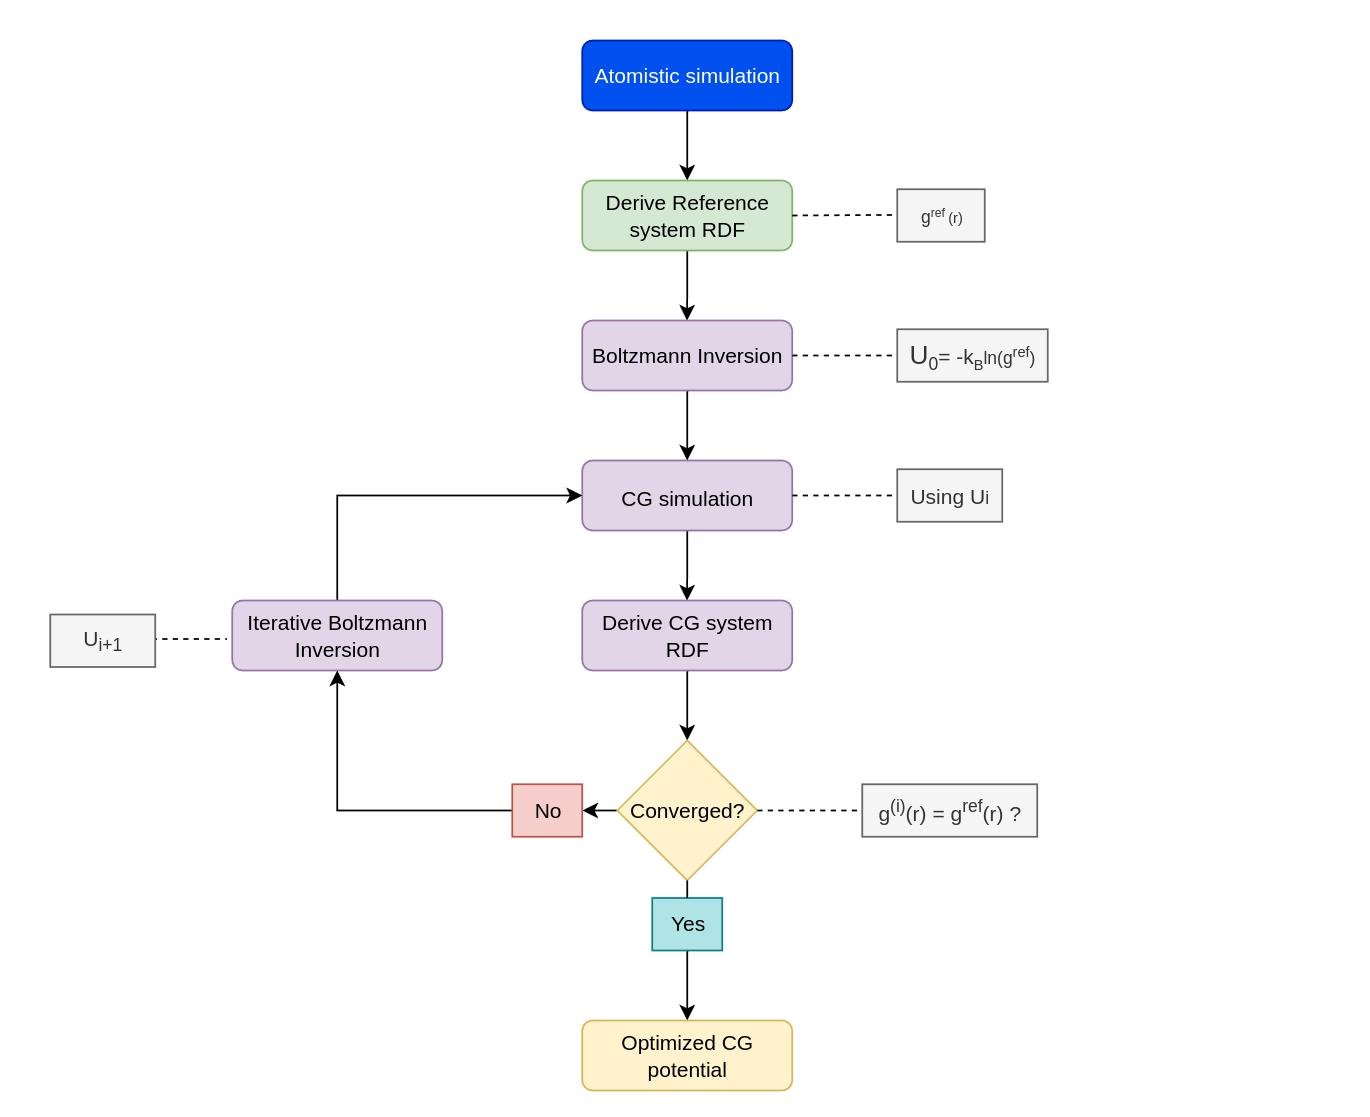
\includegraphics[width=0.9\textwidth]{flowchart_custom.jpg}
                \caption{Flowchart of the Iterative Boltzmann Inversion. Colours refer to different software used for the depicted step. Blue: GROMACS, Green: Python, Purple: MagiC.}
                \label{fig:ibi}
            \end{figure}
        
            The algorithm of the IBI process can be seen in \ref{fig:ibi}. First off the RDFs of the ion pairs in the reference system is required as input, which is derived after performing the atomistic simulation. The next step is the direct Boltzmann inversion, which gives us the starting interaction potential based on the following equation:
            \begin{equation}
                U_0 = -k_B T \ln(g^{ref}(r)),
            \end{equation}
            This step is labeled as the Boltzmann Inversion. Using this potential a simulation of the CG system is performed, from which the RDFs $g^{(i)}(r)$ (one function pair interaction pair, in our case a total of 3 such pairs) are derived, where the index $i$ implies in which iteration step the process is. Next the convergence criterion is evaluated, if $g^{(i)}(r) = g^{ref}(r)$, this means that the effective potentials of the CG system accurately reproduce the statistics of the RS. If the RDF has not converged to that value, then the iterative Boltzmann inversion takes place, where the used effective potential is updated based on the following equation:
            \begin{equation}
                U_{i+1}(r) = U_i(r) + k_B T \ln(\dfrac{g^i(r)}{g^{ref}(r)}).  
            \end{equation}
            The updated potential is used to perform a new simulation, from which a new statistic $g^{(i+1)}$ is derived. Again the new RDF is compared to that of the RS. This process continues until the $n-$th step where $g^{n}$ has converged to the RDF of the RS. Typically it is expected that the process needs around 10 iterations until convergence is reached, which is considered rather fast and therefore has the benefit of saving up computational resources. 
            
        %reith and ruhle for this
        
        
    \subsection{Implementation}
    %make a graph for this
    %IBI according to Ruhle needs smoothing an extrapolation... hmmm
        \label{implementation}

                \begin{figure}[H]
                    \centering
                    \includegraphics[width= 0.8\textwidth]{Implementation_hori.jpg}
                    \caption{Flowchart depicting the implementation on a software level. Fully coloured boxes depict the software used, while transparent ones the files used as input and generated as output at each stage.}
                    \label{fig:implem_flowchart}
                \end{figure}
                
                The implementation of the above algorithm required the use of a variety of software. The initial input was a trajectory file from a simulation of the reference system performed in GROMACS \cite{Gromacs}. The trajectory file contained 501 steps with a $\Delta t = 40 ns$ for 40 particles. On a self developed code in Python, based on an algorithm written by D. Frenkel \& B. Smit \cite{Frenkel}, we derived the RDFs of the ion particles. Afterwards some data processing was performed on the resulting functions, specifically smoothing as is necessary when using IBI \cite{Ruhle}. In \ref{fig:rdf_Na-Cl}\ref{fig:rdf_Na-Na}\ref{fig:rdf_Cl-Cl}, we see the reference system RDFs of the ion pairs as obtained from the trajectory file with Python and after performing the required smoothing on it.
                %or should I give the reference rdf ? or MagiC end RDF?

                The resulting RDF is then given as input in MagiC \cite{Magic} for RDF of the reference system in order to perform the IBI as seen in \ref{fig:ibi} (steps colored in purple). A variety of parameters can be set manually in MagiC, with the most important being the amount of iteration steps. As mentioned before typically 10 steps are needed, but in our case we see converge being reached after around 20 steps.

        
\section{Results}

    \label{Results}

    In this section the initial radial distribution functions are presented which were calculated with a Python script and the primary results of the effective potentials derived with MagiC. The units of x-axis is Ångström, while the y-axis is Joules for Potentials $U(r)$ and density of the number of particles for RDFs $g(r)$.

    
    
    

    \subsection{Radial distribution function}
        \label{r:rdf}

        In this section the results for the RDFs of ion pairs are being depicted, which are derived from the trajectory obtain from an atomistic simulation on GROMACS.
        
        In figure \ref{fig:rdf_Na-Cl}, in te top graph we see the raw data obtained by using the Python algorithm on the trajectory data, which already gives us a clear impression of the RDF. In the bottom graph we have performed some data processing, including smoothing which is required for the IBI. As a side effect of the smoothing process, the first peak has been reduced in size. The red line on $y = 1$ is there to guide the eye and see how the RDF converges to 1.
    
        \begin{figure}[H]
            \centering
            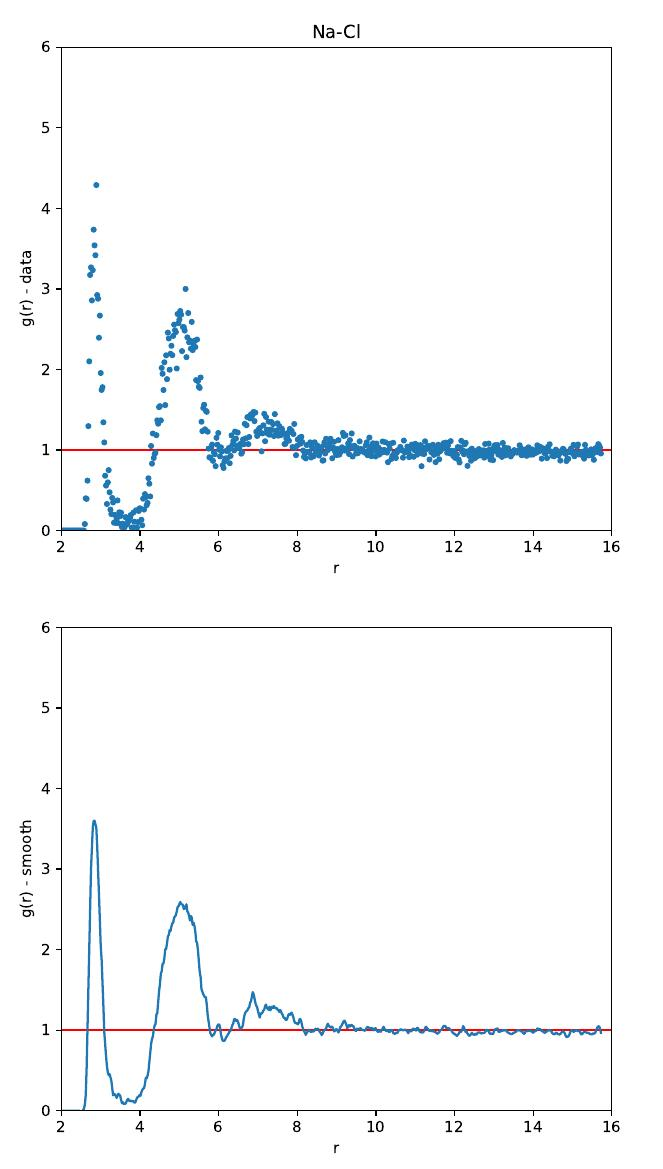
\includegraphics[width = 0.7\textwidth]{RDF-NaCl.jpg}
            \caption{RDF of Na-Cl.}
            \label{fig:rdf_Na-Cl}
        \end{figure}

        In the following figures \ref{fig:rdf_Na-Na}, \ref{fig:rdf_Cl-Cl}, the results of the RDF for the Na-Na and Cl-Cl pairs are depicted.

    \begin{figure}[H]
            \centering
            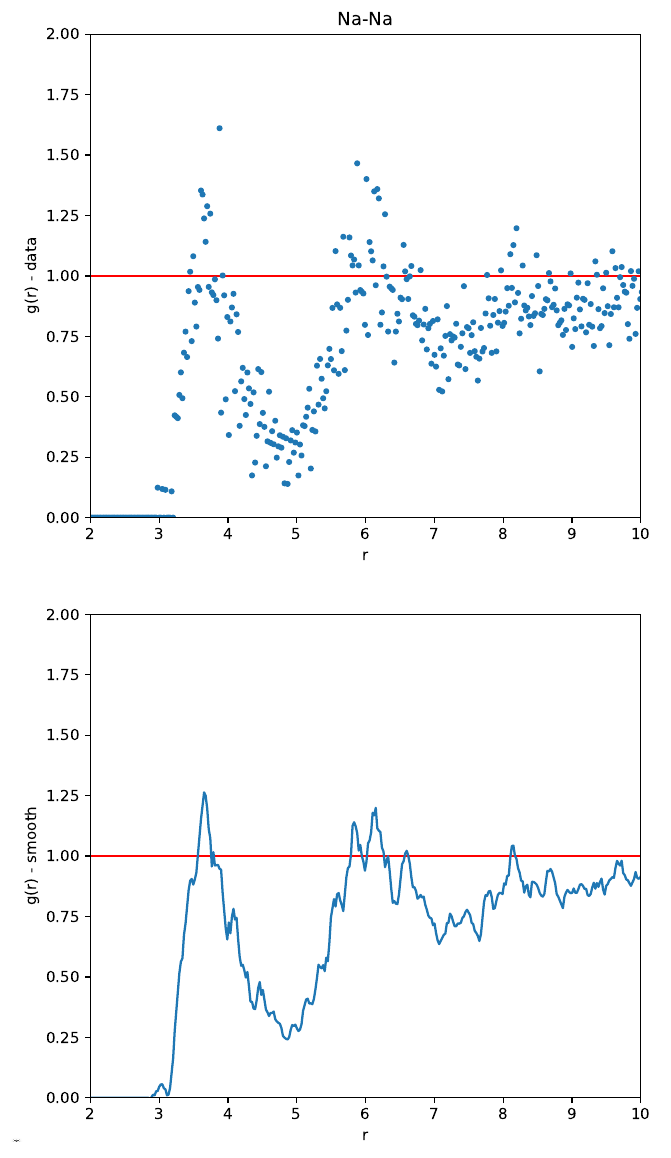
\includegraphics[width = 0.7\textwidth]{RDF-NaNa.png}
            \caption{RDF of Na-Na.}
            \label{fig:rdf_Na-Na}
    \end{figure}

    \begin{figure}[H]
            \centering
            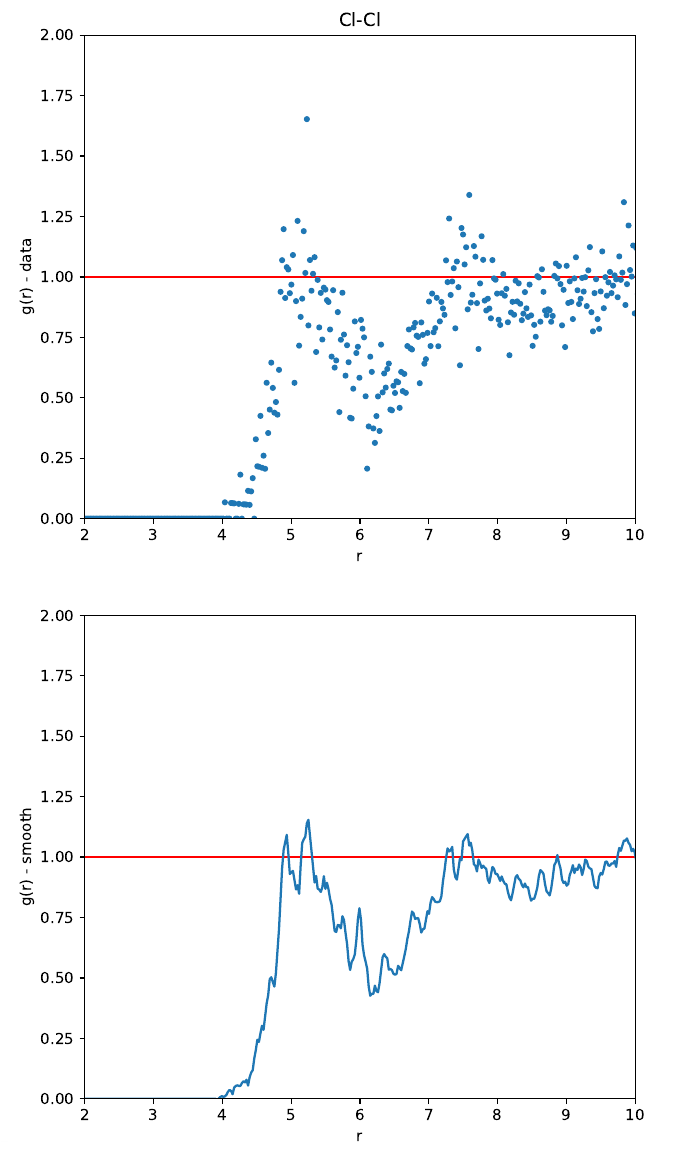
\includegraphics[width = 0.7\textwidth]{RDF-ClCl.png}
            \caption{RDF of Cl-Cl.}
            \label{fig:rdf_Cl-Cl}
    \end{figure}
    
    \subsection{Ion-ion effective potentials at different iteration steps}
        \label{r:pot}

        The potentials are plotted at their different iteration stages, up to the final 20th iteration, for better understanding of how the potential converge. The concentration of the ions is of 1M. The last graphic, contains the effective potential of Na-Cl \ref{fig:Na-Cl-iter}, which we can see changed profoundly from step 5 through step 14 and still displays a significant change from step 14 to 20 in the first peak. Quantitatively that is a ~30\% increase. The graphics for Na-Na and Cl-Cl interaction can be found in the appendix \ref{fig:Na-Na-iter} and \ref{fig:Cl-Cl-iter} respectively.
        
        

        \begin{figure}[H]
            \centering
            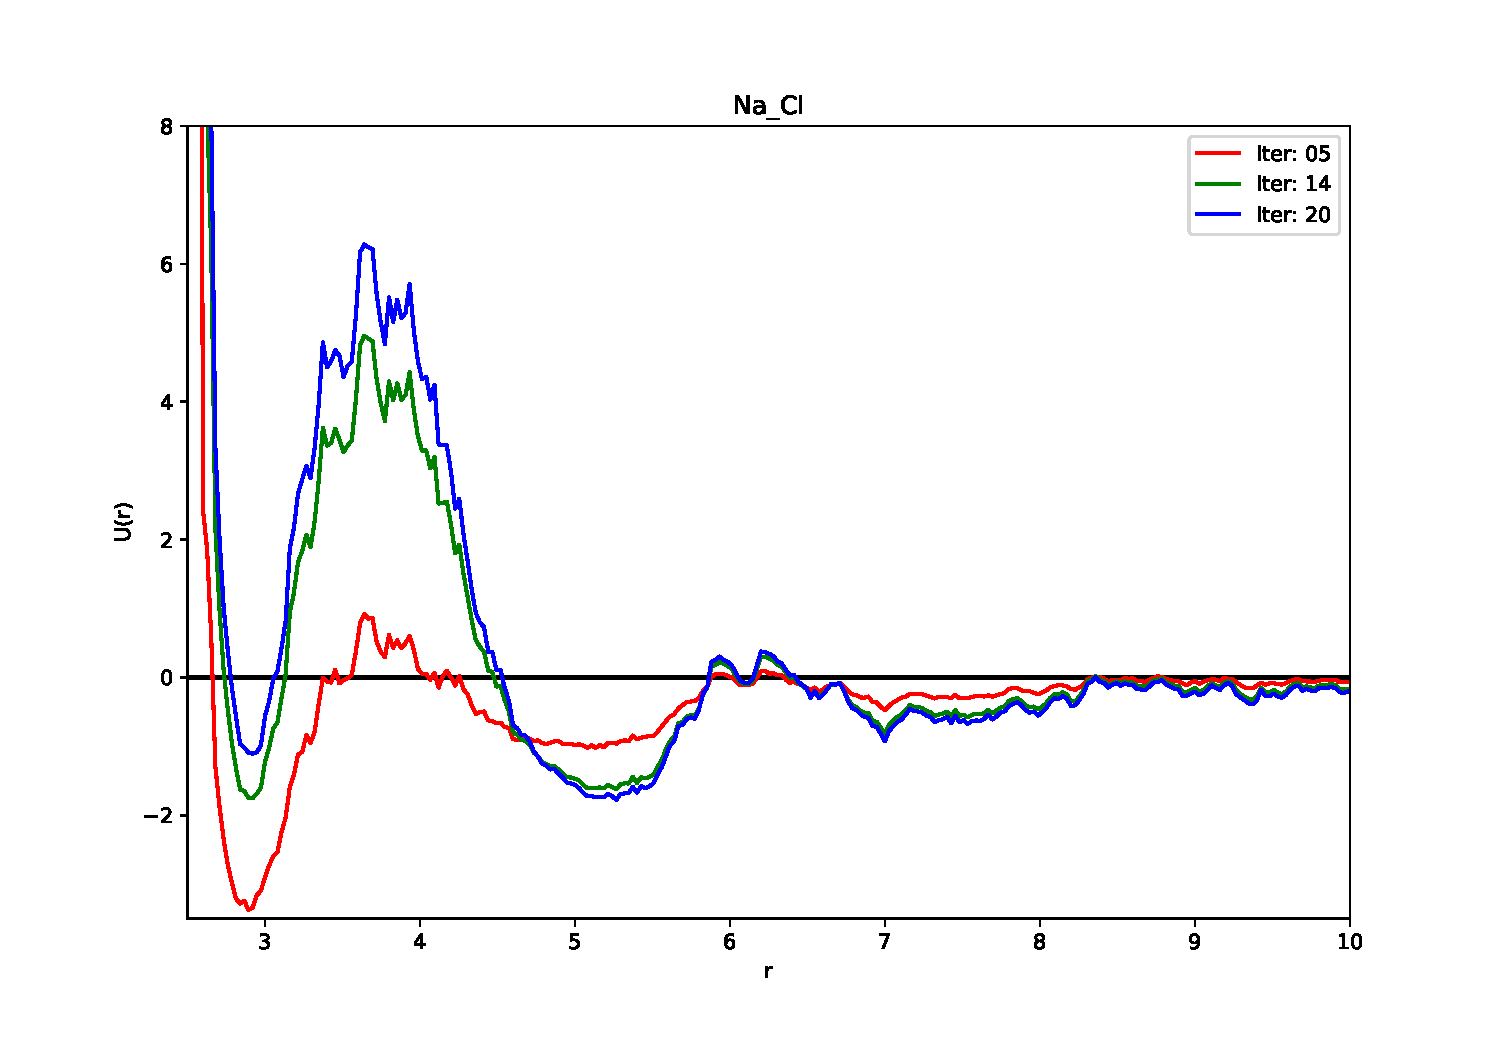
\includegraphics[width = 0.7\textwidth]{iters_conv_Na_Cl.pdf}
            \caption{Na-Cl Potential in different iterations stages (Red: 5, Green: 14, Blue: 20).}
            \label{fig:Na-Cl-iter}
        \end{figure}
%1.0 Mol

%Na-Na different stages
%Cl-Cl
%Na-Cl

    \subsection{All pair potentials}
        
        \begin{figure}[H]
            \centering
            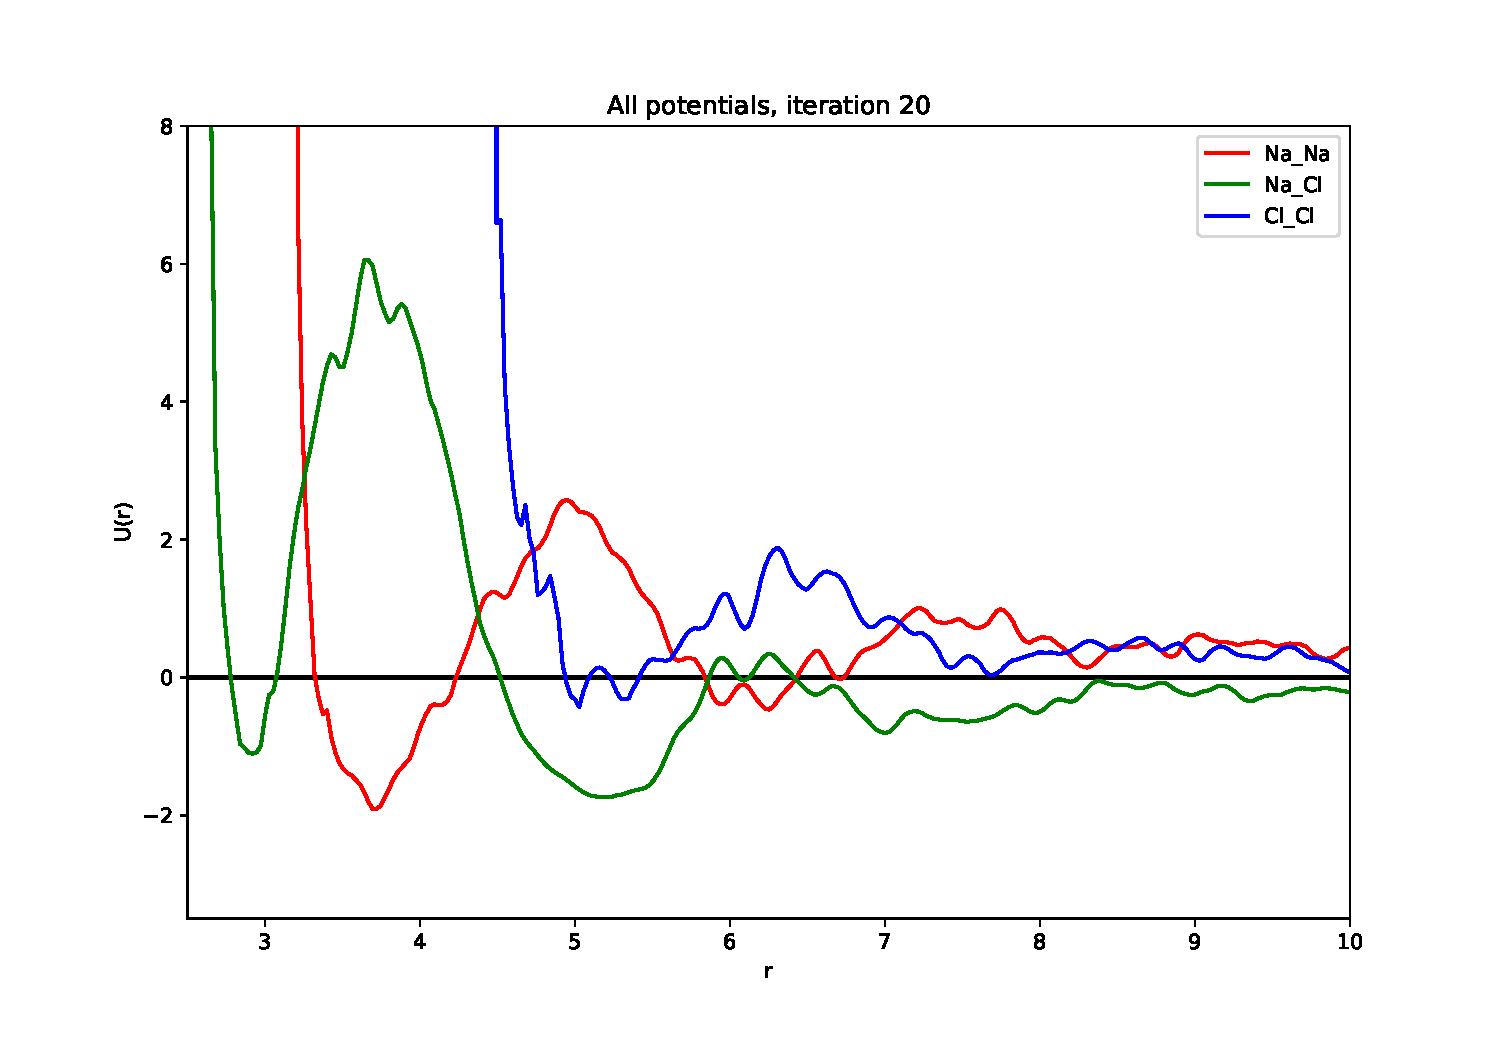
\includegraphics[width = 0.8\textwidth]{iters_all_20_smoothed.pdf}
            \caption{Effective potentials of all ion-ion pairs after 20 iterations with convergence reached, with the data being smoothed. Red: Na-Na, Green: Na-Cl, Blue: Cl-Cl}
            \label{fig:allpot_smooth}
        \end{figure}

        The converged effective potentials of the three ion pairs can be seen in figure \ref{fig:allpot_smooth} above. Obtained with MagiC after 20 iterations, these are the optimal CG potentials. A figure displaying all these potentials separately can be found in the appendix \ref{fig:allpot_unproc_separate}.



\section{Outlook}
%Results comparison with other such data
%Comparison to different molarity
%Comparison to different software results, different method

    The application of the Iterative Boltzmann Inversion for the derivation of effective ion-ion potentials in aqueous electrolytes has been overall successful. We managed to obtain the optimized CG potentials for a concentration of 1M in a box with dimensions 31.427$\si{\angstrom}$. Our goal is to evaluate the effectiveness of the methods implemented, as well the behavior of the effective potentials under different conditions. In order to evaluate the quality of the results we have obtained we will be comparing them to the results of other reported works, since we have not obtained results from different simulations ourselves in this work. When doing so, we will be looking at three attributes. First the overall shape of the graphs obtained. Secondly the proportions between peaks, i.e if the first peak is two times larger than the second in our results, we expect it be so as well in the other works and vice versa, or at the very least the relation of which peak is larger should be preserved, under the assumptions that the simulations were both performed under the same conditions. Thirdly the numerical values of the effective potentials, although those can vary a lot depending on the temperature, box size and concentration and are thus of less importance in general but can offer some insight \footnote{Also because the potentials can be determined up to an additive constant as we will see later \cite{Ruhle}}. We will also analyze how different conditions change or could affect the effective potentials as seen in the reported works.

    
    \label{outlook}
    \subsection{Comparison to other results}

        First the RDF obtained for Na-Cl as seen in figure \ref{fig:rdf_Na-Cl}, has shape and curves that are similar to those reported in \cite{Lyubartsev1} and \cite{Lyubartsev2}. The main difference is exhibited at the intensity of the peaks, especially the first one, which must be a caused by setting a smaller box (approx. 19 $\si{\angstrom}$ ) for the simulation in the former work. Comparing the RDF of Na-Cl with the latter work, the shape and intensities match a lot better, in which the concentration of 1M and a box of size 39.02 $\si{\angstrom}$ were used \footnote{Since the parameters used in the second work our closer to ours, we will be focusing our comparisons to that one}. Nevertheless, it seems that the relation between the first and second peak is not the same in our work as in the reported work, we will see how this could affect the effective potential later. Despite this detail, the RDFs seem to match and this is a good indicator, telling us that the simulation by GROMACS was performed well and most importantly that the algorithm for deriving the RDF was implemented on Python properly. Therefore we can make a cleaner comparison for the derived effective potentials later on. It should also be noted that the concentration, whether 0.8M, 1M, or 2.2 M, has a visible albeit minor influence on the shape of the function and the intensity of the peaks as seen in the reported works.

        Secondly a qualitative comparison of the Na-Cl effective potentials produced here with the ones in the literature gives an overall similar shape albeit with some differences in the proportions. These differences affect the the physical interpretation of the two results. In our case the magnitude of the first dip is larger than the second one, whilst in \cite{Lyubartsev2} the second dip is deeper than the first. An important note on this is that the effective potentials can only be determined up to an unknown constant (\cite{Ruhle} p.3213), but this constant would result to just a displacement of the graph along the y-axis and not alter the proportions. Therefore this unknown constant is not the culprit for the discrepancy, since it is the relation between the infima of the potentials that is different.
        
        This difference is significant since the physical interpretation would imply contradictory results for the distance $r$ at which point the potential is expected to have lowest energy. Since the discrepancy does not seem to originate from a difference in the scaling of the two graphs. Another explanation \textit{could} stem from the fact that in our case we used the IBI method as opposed to Inverse Monte Carlo in the reported work. As mentioned in \cite{Ruhle} "small changes in the radial distribution function often lead to big changes in the pair potential". As we saw before the first peak of our RDF is smaller than the one in the reported work, what could be at fault is the smoothing performed on Python using different parameters and methods than in the literature. It can be argued that the smoothing process with Python affected the magnitude of the peaks and dips more than the methods used in the reported work, as we can also see in figure \ref{fig:rdf_Na-Cl}.

        As for the Na-Na and Cl-Cl interaction potentials, the results seem to be more consistent with the literature results. The shape is almost identical and the proportions of the peaks and dips between the results is maintained. For that reason the different box sizes used for the simulations are probably not the cause for the discrepancy in the Na-Cl results.


        %dont forget to mention the additive constant

    \subsection{Conclusions \& Future direction}
    
    Ideally we would want a work like this to stand on its own. That could be done by producing results for different concentrations, box sizes and methods used. It would be of great interest in such a framework to perform simulations with different parameters other than molarity (e.g box size) and see how those can affect the effective potentials of the ion-ion interactions. The effective potentials seem to not change much with the concentration, at least under the given conditions (box size, pressure, temperature) seen in the reported works. This is clearly demonstrated in \cite{Lyubartsev2}, where despite doubling the molarity from 0.5M to 1.0M and observing changes in the RDFs, it yields close to no change in the interaction potentials. The changes are only marginal, that could even be interpreted as within the boundaries of standard deviation. In this case scenario it would be interesting to see how IBI would perform under these changes, since it has been claimed to be more sensitive under changes in the RDF.

    Furthermore on the software implementation side of these methods, experience has shown that it is highly preferred to use a more unified framework of software, where different settings and outputs can be streamlined with as less hassle as possible. In the same fashion as in the work of Rühle et al. \cite{Ruhle} where VOTCA was implemented, an overarching toolkit for computational physics purposes. For unknown reasons, MagiC was incapable of performing the IBI for an RDF obtained for different parameters, namely for a concentration of 0.5M. Although the process was repeated in an identical manner to the case of 1M. Additionally it failed in producing results using the Inverse Monte Carlo method with the same input data as for the IBI for the case of 1M. These limitations resulted in a reduction of the scope of the work.

    On a final note, it should be taken into consideration that the IBI method while useful in this simple case scenario, is not reliable by itself when having more complex systems. The reason for that is that it does not take into account cross-correlation terms when updating the potentials. Meaning that the potential of Na-Na interaction does not take into account that of Na-Cl. Additionally there may be convergence issues for the potentials, those can be compensated by multiplying the update term of the potential with a factor $\eta \in (0, 1)$ \cite{Ruhle}. For that reason opting for a different method, e.g Inverse Monte Carlo, which is viable for a wider array of systems and therefore more applications should be taken into consideration. Nevertheless IBI is still preferred in certain simple cases, for its speed and ease of implementation.

\begin{thebibliography}{9}

\bibitem{Frenkel}
Understanding molecular simulations from algorithms to applications, Daan Frenkel \& Berend Smit, Academic Press, 2nd Edition.

\bibitem{Rapaport}
The Art of Molecular Dynamics Simulations, D.C. Rapaport, Cambridge University Press, 2nd Edition.

\bibitem{Lyubartsev1}
Calculation of effective interaction potentials from radial distribution functions: A reverse Monte Carlo approach, Physical Review E, 1995.

\bibitem{Lyubartsev2}
Evaluation of effective ion-ion potentials in aqueous electrolytes, Alexander P. Lyubartsev \& Stjepan Marcelja, Physical Review E, \url{https://doi.org/10.1103/PhysRevE.65.041202}.

\bibitem{Reith}
Deriving effective Mesoscale Potentials from Atomistic Simulations, Reith et al, Wiley Periodicals, 2003.

\bibitem{Ruhle}
Versatile Object-Orienten Toolkit for Coarse-Graining Applications, Rühle et al, JCTC, 2009.

\bibitem{Magic}
Alexander Lyubartsev,
Alexander Mirzoev, \\
\url{http://www.fos.su.se/~sasha/magic/}, \\
\url{https://bitbucket.org/magic-su/magic_tutorials/src/master/}.

\bibitem{Gromacs}
\url{https://www.gromacs.org/}.

\bibitem{GitHub}
\url{https://GitHub.com/iasonq/lab-comphys-statmech-2}.

\end{thebibliography}

\newpage

\appendix

\section{Appendix}
\label{appendix}
    \subsection{GitHub code}
        \label{a:code}

        The following algorithm is a snippet of the code used to derive the RDF of an ion pair. This code is based on algorithm provided by D. Frenkel \& B. Smit \cite{Frenkel}. The full code can be found on GitHub \cite{GitHub}.
        
        \begin{lstlisting}[language=Python, caption=Sample from rdf.ipynb]
###1st part
def rdf(g, ngr, cell, data, delg, npart, chunk, pair, set):

    if pair == 0: #Na-Na

        for k in range(0, npart, chunk):
            ngr = ngr + 1 
            for i in range(k+0, k+chunk-1-set): 
                for j in range(i+1, k+chunk-set ):
                    r = data[i]-data[j]
                    #implement periodic boundary conditions
                    r = r - cell*np.round(r/cell) # ok
                    r = np.linalg.norm(r) # ok
                    if r <= cell/2: 
                        l = int(r/(delg))
                        g[l] = g[l] + 2
    elif Na-Cl:
        ...
    elif Cl-Cl:
        ...
    
    return g, ngr
    
###2nd part 
    
def grdf(g, delg, ngr, bins, cell, pair, set):

    apart = set 
    rho = apart/(cell**3)
    if pair == 2:
        rho = 2*rho

    r = []
    for i in range(0, bins): 
        r.append(delg*(i+0.5))
        vol = ((i+1)**3  - i**3 )*delg**3 
        nid = (4/3)*np.pi*vol*rho
        g[i] = g[i]/(ngr*apart*nid)  
    return g, r

    
    \end{lstlisting}
        
    \newpage
    \subsection{Potentials}
        \label{a:pot}
         In the following figures the effective potentials of Na-Na and Cl-Cl interactions can be seen for iteration steps 5,14 and 20.
         
        \begin{figure}[H]
            \centering
            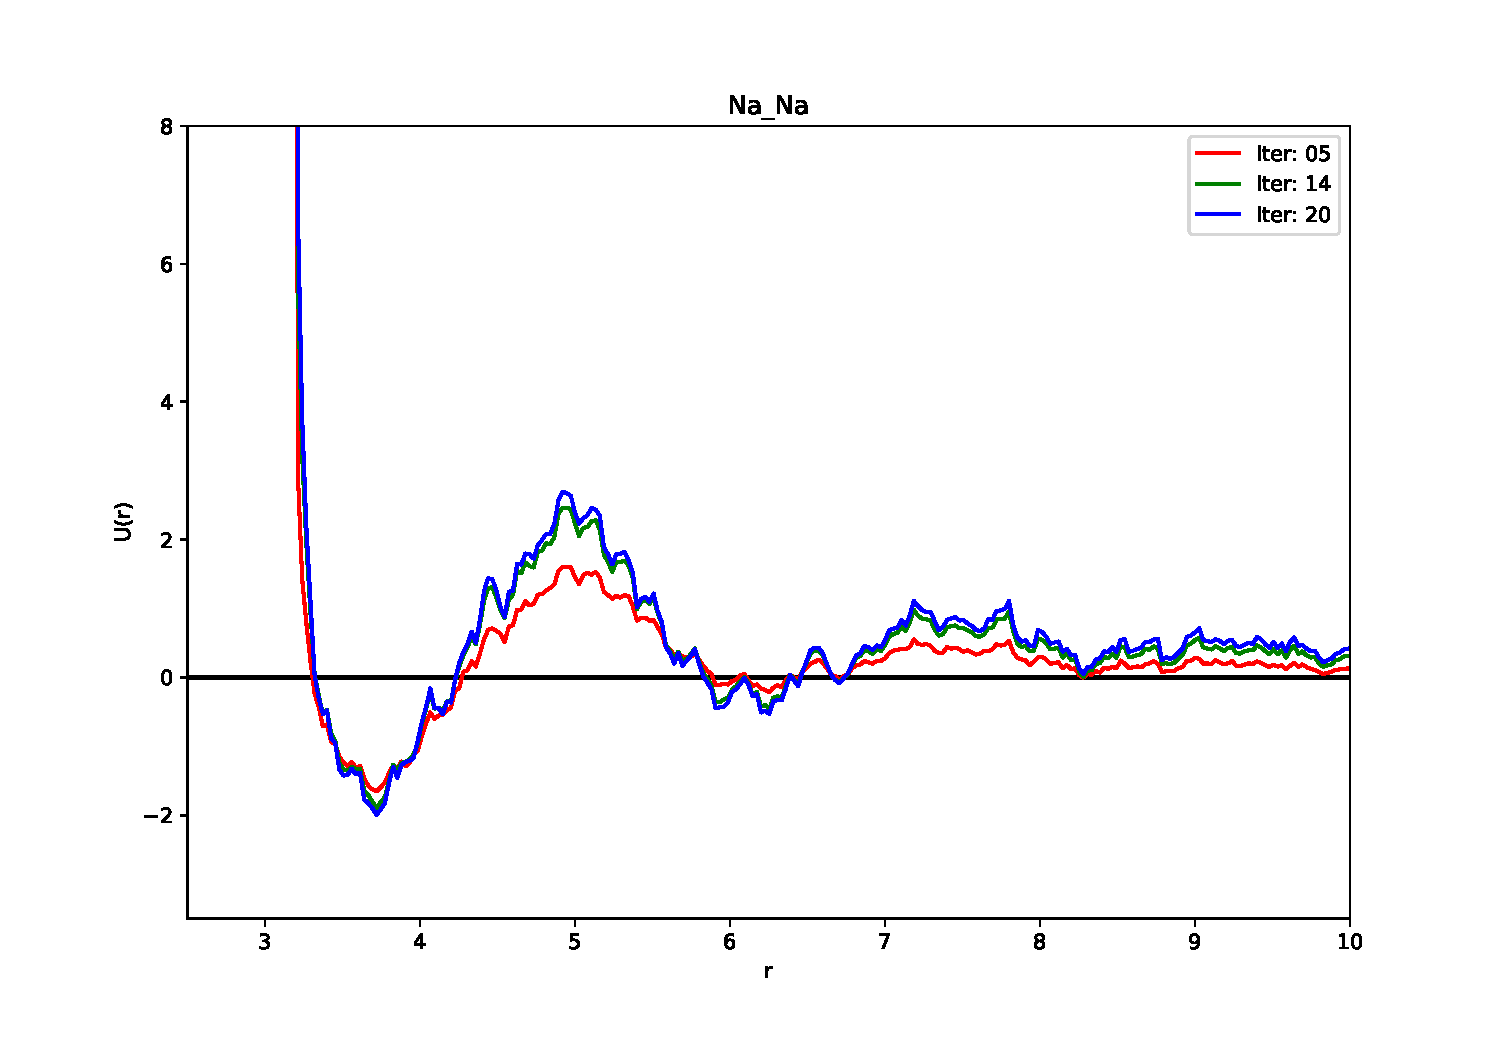
\includegraphics[width = 0.7\textwidth]{iters_conv_Na_Na.pdf}
            \caption{Na-Na Potential in different iterations stages (Red: 5, Green: 14, Blue: 20).}
            \label{fig:Na-Na-iter}
        \end{figure}

        \begin{figure}[H]
            \centering
            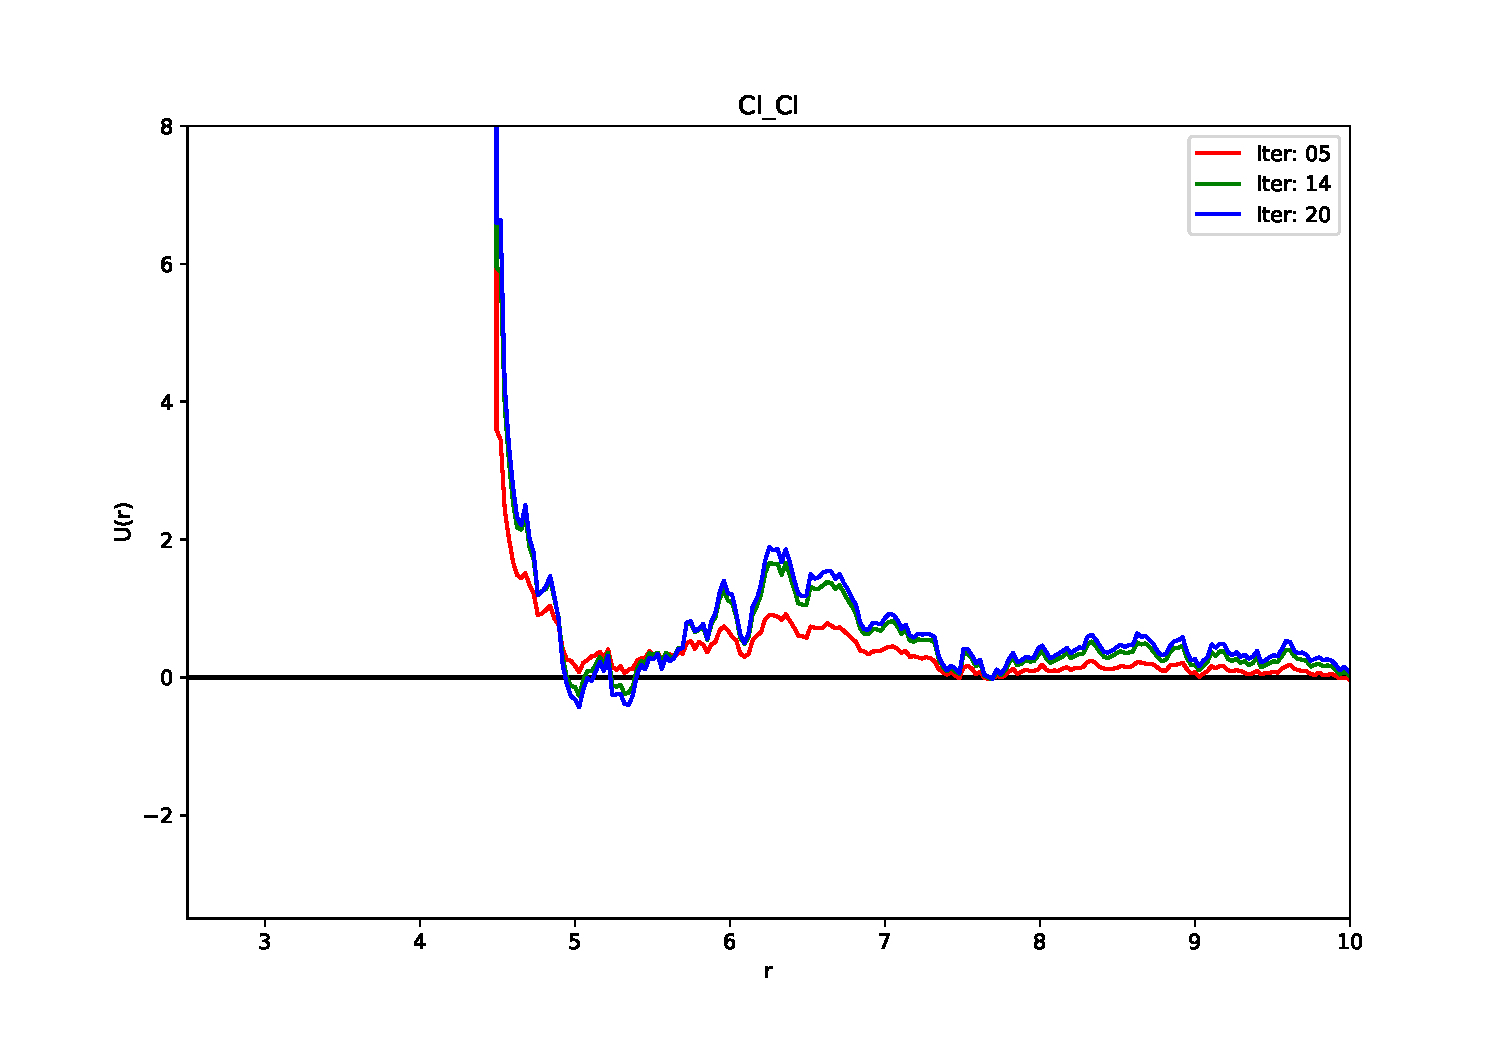
\includegraphics[width = 0.7\textwidth]{iters_conv_Cl_Cl.pdf}
            \caption{Cl-Cl Potential in different iterations stages (Red: 5, Green: 14, Blue: 20).}
            \label{fig:Cl-Cl-iter}
        \end{figure}

        In the following figure the raw data can be seen from which the smoothed data \ref{fig:allpot_smooth} is derived, this is the output given by MagiC when performing the IBI.
        
        \begin{figure}[H]
            \centering
            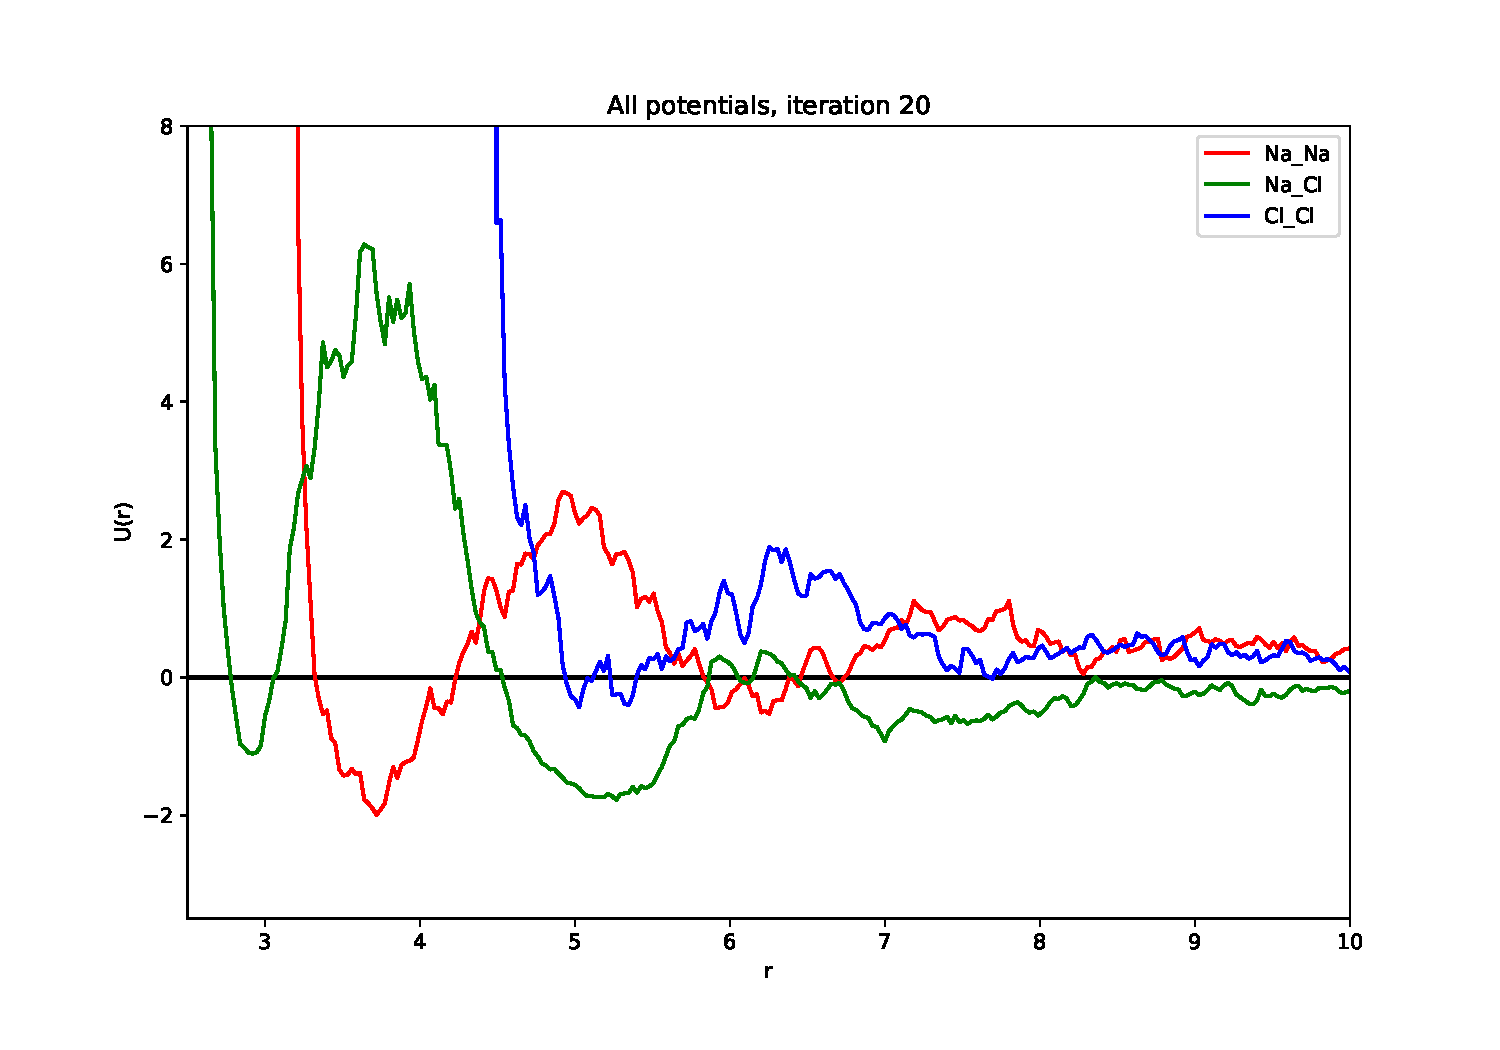
\includegraphics[width = 0.8\textwidth]{iters_all_20.pdf}
            \caption{Effective potentials of all ion-ion pairs after 20 iterations with convergence reached, unprocessed.}
            \label{fig:allpot_unproc}
        \end{figure}
        
        \newpage
        \subsubsection{All ion pair optimized CG effective potentials}
        The following figure is a collection of all three ion pair effective potentials after convergence has been reached. 
            \begin{figure}[H]
                \centering
                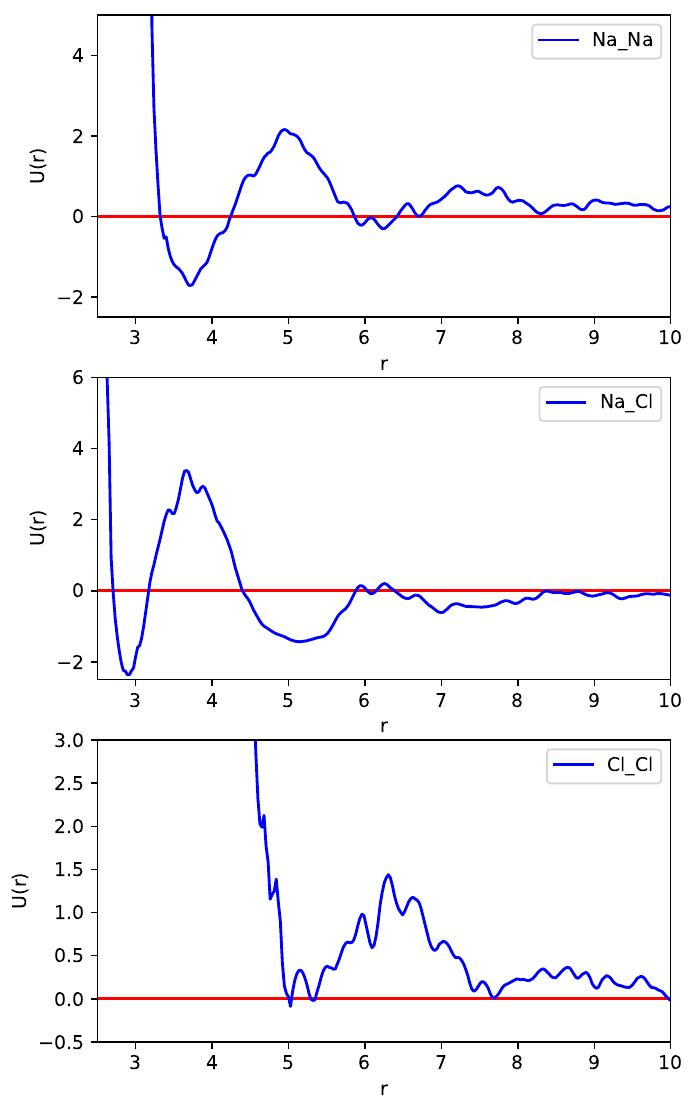
\includegraphics[width = 0.8\textwidth]{All_pots_iter20_separate_a.jpg}
                \caption{Effective potentials of all ion-ion pairs after 20 iterations with convergence reached, smoothed, separately. Displaying from top to bottom: Na-Na, Na-Cl, Cl-Cl.}
                \label{fig:allpot_unproc_separate}
            \end{figure}

        
\end{document}